\chapter{Méthodologie et résultats expérimentaux}
\label{ch:xp}

Après avoir décrit les algorithmes, ce chapitre les met à l'épreuve sur des
données réelles. On commence par préciser le protocole (instance, requêtes,
métriques) qui garantit une comparaison équitable, puis on présente les
résultats : de l'exemple visuel d'un trajet parisien jusqu'à l'étude du passage à
l'échelle qui constitue le résultat central du projet.

\section{Protocole expérimental}
\label{sec:protocole}

Toutes les expériences suivent le même protocole, résumé ci-dessous :

\begin{bulletlist}
  \item \textbf{Instance :} réseau routier de Paris, 9\,235 nœuds
        (plus grande composante fortement connexe, table~\ref{tab:instance}).
  \item \textbf{Requêtes :} $N$ couples $(s, t)$ aléatoires tirés d'une graine
        fixe, \emph{identiques} pour tous les algorithmes (comparaison
        équitable). Le banc d'essai utilise $N = 200$, l'étude des landmarks
        $N = 100$, l'analyse statistique $N = 300$.
  \item \textbf{Métriques :} nœuds explorés et temps de réponse
        (\S\ref{sec:metriques}), plus le contrôle d'optimalité contre Dijkstra sur
        chaque requête.
  \item \textbf{Reproductibilité :} toutes les figures et tous les tableaux sont
        produits par les scripts de \texttt{scripts/}, à graine fixe et à partir
        d'un extrait de carte mis en cache.
\end{bulletlist}

\section{Région explorée par algorithme : l'exemple fil rouge}
\label{sec:filrouge}

L'exemple fil rouge est un trajet réel à plusieurs étapes :
\textbf{Université Paris Dauphine -- PSL $\to$ PariSanté Campus $\to$ ENS -- PSL
(Rue d'Ulm) $\to$ PSL (Rue Mazarine)}, soit 13{,}91~km, résolu comme trois legs de
plus court chemin consécutifs (\S\ref{sec:multistop}). La
figure~\ref{fig:multistop} montre, par algorithme, tous les nœuds réglés sur
l'ensemble du parcours (la « tache » colorée) et la route rendue (rouge) ; les
marqueurs sont le départ (vert), les deux arrêts intermédiaires (losanges
oranges) et l'arrivée (carré rouge).

\begin{figure}[H]
  \centering
  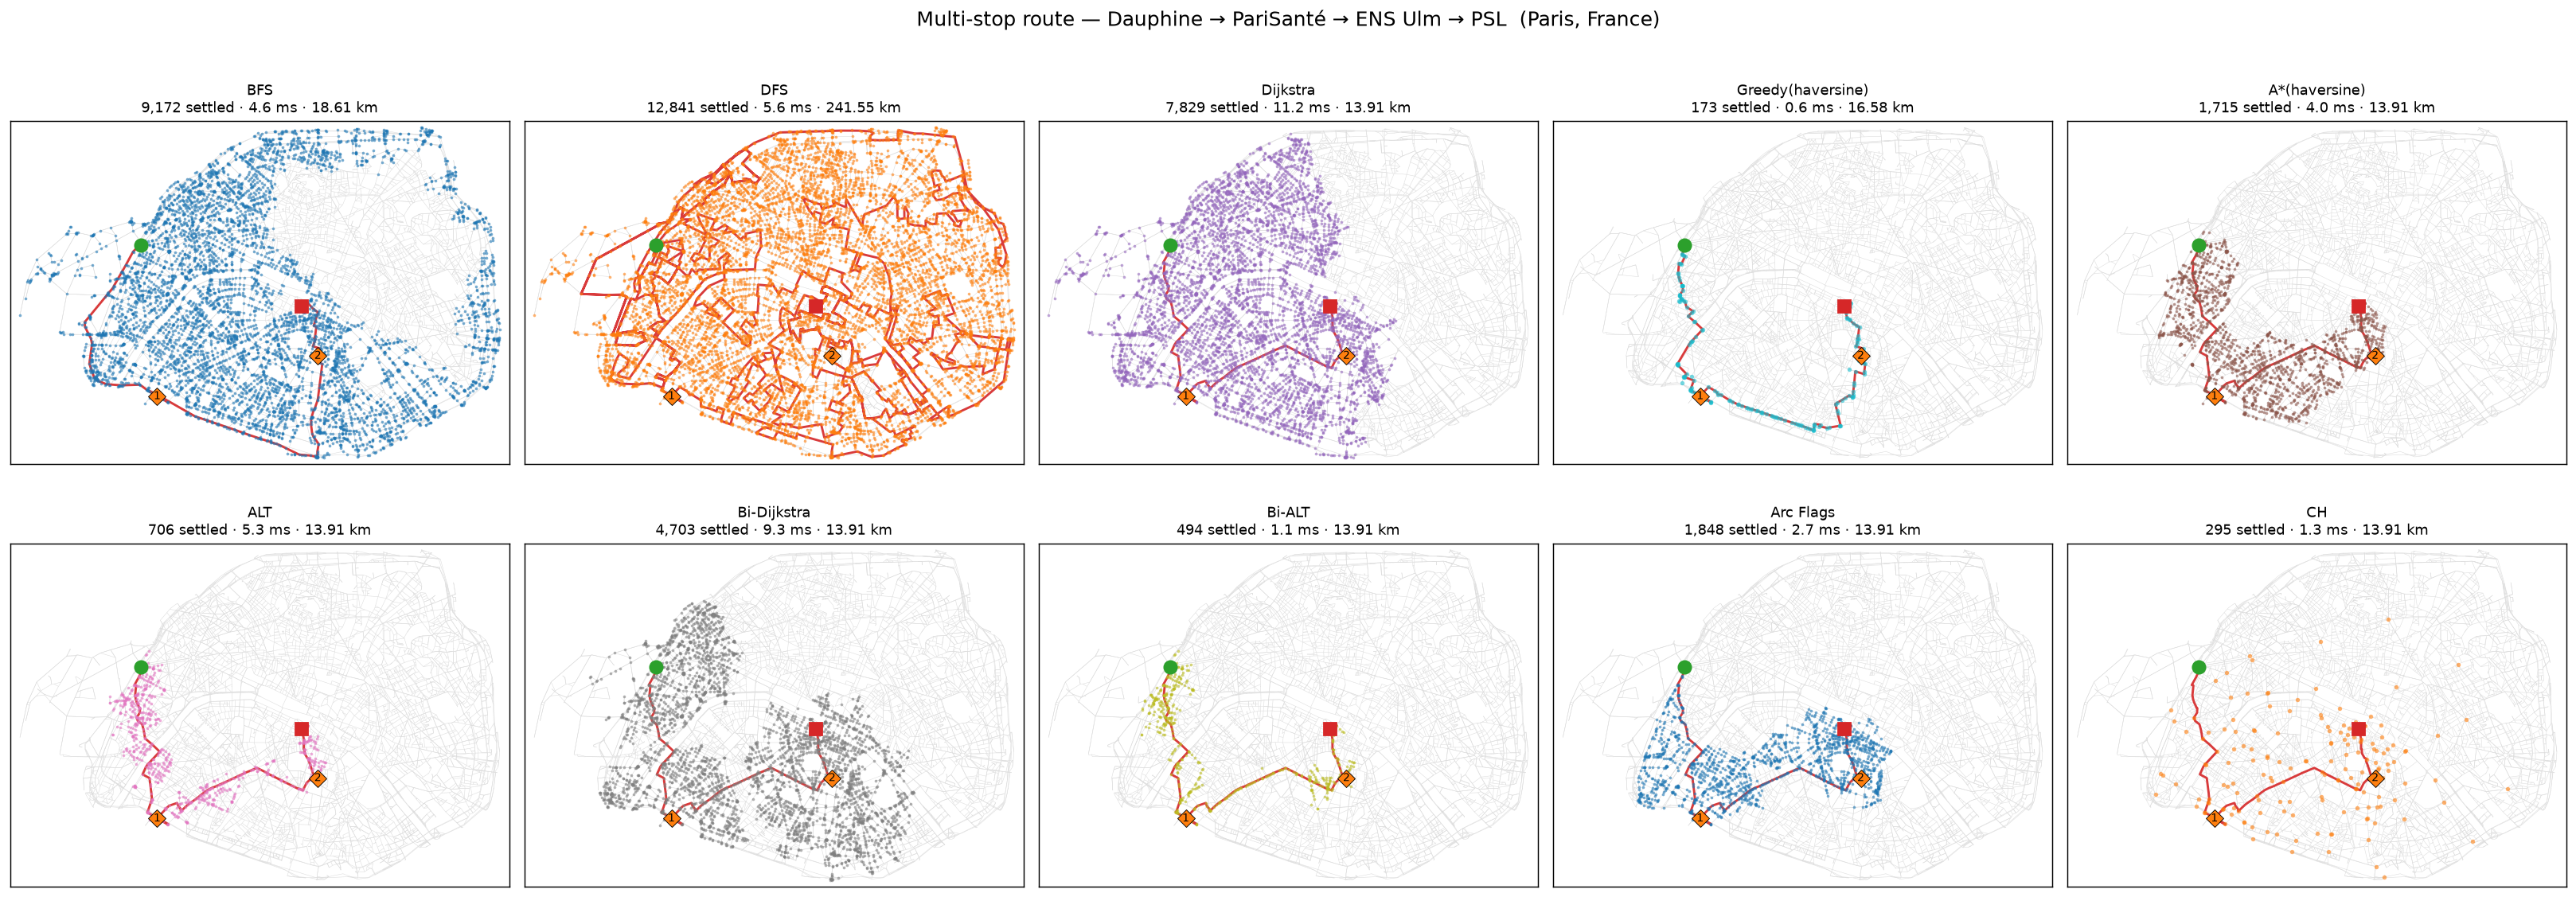
\includegraphics[width=\textwidth]{figures/multi_stop_comparison.png}
  \caption[Régions explorées par les dix algorithmes]{Régions explorées par les
  dix algorithmes sur le trajet fil rouge (Dauphine $\to$ PariSanté $\to$ ENS
  $\to$ PSL). La tache colorée est l'ensemble des nœuds réglés ; la ligne rouge
  est la route rendue.}
  \label{fig:multistop}
\end{figure}

C'est le résultat le plus éloquent : \textbf{BFS/DFS} inondent la carte (la route
de DFS atteint 241~km) ; \textbf{Dijkstra} couvre une vaste région (7\,829
nœuds) ; \textbf{A*} la resserre en ellipse (1\,715) ; \textbf{ALT} en un mince
corridor (706, \textbf{11$\times$} moins) ; les méthodes
\textbf{bidirectionnelles} forment deux taches qui se rejoignent (Bi-ALT : 494) ;
et les \textbf{Contraction Hierarchies} règlent le moins de nœuds de tous (295,
\textbf{26{,}5$\times$}), en une \emph{nuée} de nœuds pivots. \textbf{Greedy}
n'en règle que 173 mais rallonge la route de 19\,\% : le prix de l'abandon de
l'optimalité.

\paragraph{Version animée.} Un GIF (\texttt{run\_multi\_stop.py -{}-gif})
montre les taches se former dans l'ordre réel d'expansion, tous les panneaux au
même rythme : les algorithmes frugaux (ALT, Bi-ALT, Greedy) achèvent le trajet et
s'arrêtent quand Dijkstra et Bi-Dijkstra brassent encore la ville. La
figure~\ref{fig:gif-still} embarque cette animation ; à défaut d'un lecteur
exécutant le JavaScript d'Adobe, le GIF s'ouvre aussi
\href{https://github.com/sepanta007/Problem_Modeling/raw/HEAD/results/exploration.gif}{directement}
et s'anime dans un navigateur (\texttt{results/explora-\\tion.gif}).

\begin{figure}[H]
  \centering
  \animategraphics[width=\textwidth,autoplay,loop,poster=37]%
    {12}{figures/anim/frame-}{0}{59}
  \caption[Animation de l'exploration]{Animation de l'exploration
  (\texttt{exploration.gif}, embarquée) : elle défile automatiquement en boucle
  dans Adobe Acrobat / PDF-XChange, et reste figée sur une image ailleurs. À un
  instant donné, ALT et Bi-ALT ont déjà terminé alors que Dijkstra et Bi-Dijkstra
  explorent encore, toutes les taches progressant au même rythme.}
  \label{fig:gif-still}
\end{figure}

\section{Banc d'essai agrégé (200 requêtes)}
\label{sec:bench}

Au-delà d'un trajet particulier, on mesure maintenant chaque algorithme sur 200
requêtes aléatoires, afin d'obtenir une vue moyenne et fiable de son coût. La
figure~\ref{fig:benchmark} en donne un aperçu visuel et le
tableau~\ref{tab:benchmark} les chiffres exacts, que l'on commente ensuite.

\begin{figure}[H]
  \centering
  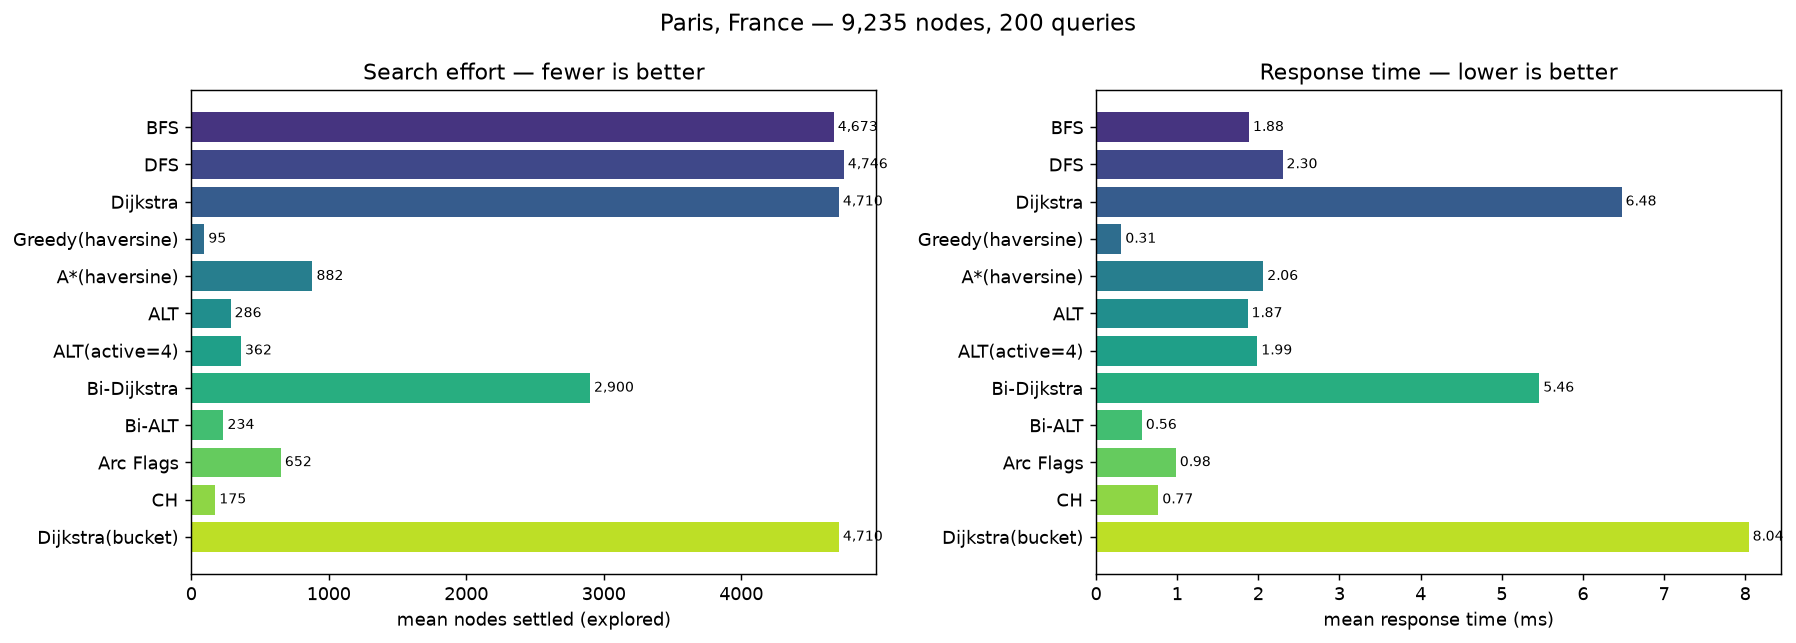
\includegraphics[width=0.95\textwidth]{figures/benchmark_summary.png}
  \caption[Synthèse du banc d'essai]{Synthèse du banc d'essai sur 200 requêtes
  aléatoires : nœuds explorés et temps moyen par algorithme.}
  \label{fig:benchmark}
\end{figure}

\begin{table}[H]
  \centering
  \small
  \begin{tabular}{@{}lrrrc@{}}
    \toprule
    Algorithme & Nœuds explorés & vs Dijkstra & Temps (ms) & Optimal \\
    \midrule
    BFS                 & 4\,673 & 1{,}0$\times$  & 1{,}89 & non ($+216\,\%$ km) \\
    DFS                 & 4\,746 & 1{,}0$\times$  & 2{,}30 & non ($+36000\,\%$ km) \\
    Dijkstra            & 4\,710 & 1{,}0$\times$  & 6{,}48 & oui \\
    Greedy (haversine)  & 95     & 49{,}6$\times$ & 0{,}31 & non ($+79\,\%$) \\
    A* (haversine)      & 882    & 5{,}3$\times$  & 2{,}06 & oui \\
    ALT                 & 286    & 16{,}5$\times$ & 1{,}87 & oui \\
    ALT (actifs $=4$)   & 362    & 13{,}0$\times$ & 1{,}99 & oui \\
    Bi-Dijkstra         & 2\,900 & 1{,}6$\times$  & 5{,}46 & oui \\
    Arc Flags ($R=32$)  & 652    & 7{,}2$\times$  & 0{,}98 & oui \\
    \textbf{Bi-ALT}     & \textbf{234} & \textbf{20{,}1$\times$} & \textbf{0{,}56} & oui \\
    \textbf{CH}         & \textbf{175} & \textbf{26{,}9$\times$} & 0{,}77 & oui \\
    Dijkstra (seaux)    & 4\,710 & 1{,}0$\times$  & 8{,}04 & oui \\
    \bottomrule
  \end{tabular}
  \caption{Banc d'essai sur Paris (200 requêtes, graine fixe). L'erreur relative
  vaut 0 pour tous les algorithmes optimaux.}
  \label{tab:benchmark}
\end{table}

\noindent Lecture du tableau :

\begin{bulletlist}
  \item \textbf{Les recherches non informées et non pondérées échouent
        bruyamment.} BFS explore autant que Dijkstra mais rend le chemin du
        \emph{moins d'arcs}, $+216\,\%$ plus long en \emph{mètres} : la raison
        concrète pour laquelle les arcs doivent être pondérés. DFS rend un chemin
        valide mais $+36000\,\%$ plus long : il n'a aucune notion de « court ».
  \item \textbf{La hiérarchie heuristique est exactement celle que prédit la
        théorie.} Parmi les algorithmes optimaux, plus d'information $\Rightarrow$
        moins de nœuds : Dijkstra (pas de $h$) $\to$ A* ($h$ géométrique) $\to$
        ALT ($h$ par landmarks). ALT explore \textbf{16{,}5$\times$} moins de
        nœuds que Dijkstra pour la route optimale identique.
  \item \textbf{Les Contraction Hierarchies explorent le moins de nœuds}
        (26{,}9$\times$) : leurs raccourcis permettent de sauter directement au
        sommet clairsemé de la hiérarchie.
  \item \textbf{Nœuds explorés $\neq$ temps.} Arc Flags explore plus de nœuds
        qu'ALT (652 contre 286) mais est \emph{plus rapide} en temps réel
        (0{,}98~ms contre 1{,}87~ms), car son travail par nœud est un simple test
        de bit plutôt qu'un maximum sur 16 landmarks. Inversement, les CH règlent
        le moins de nœuds mais sont un cheveu plus lentes que Bi-ALT car leur
        requête fait davantage par nœud (comptabilité des raccourcis,
        dépaquetage) en Python pur.
  \item \textbf{Bi-ALT est le plus rapide en temps réel} : combiner deux idées
        indépendantes (bidirectionnel + landmarks) compose leurs bénéfices.
\end{bulletlist}

\section{Effet du placement des landmarks}
\label{sec:landmark-study}

L'efficacité d'ALT dépend fortement du \emph{nombre} de landmarks et de la
\emph{stratégie} qui les place (\S\ref{sec:landmark-select}). On isole ici cet
effet en faisant varier $k$ pour les quatre stratégies. La
figure~\ref{fig:landmark-study} et le tableau~\ref{tab:landmark-study} en donnent
les résultats, dont on tire trois enseignements.

\begin{figure}[H]
  \centering
  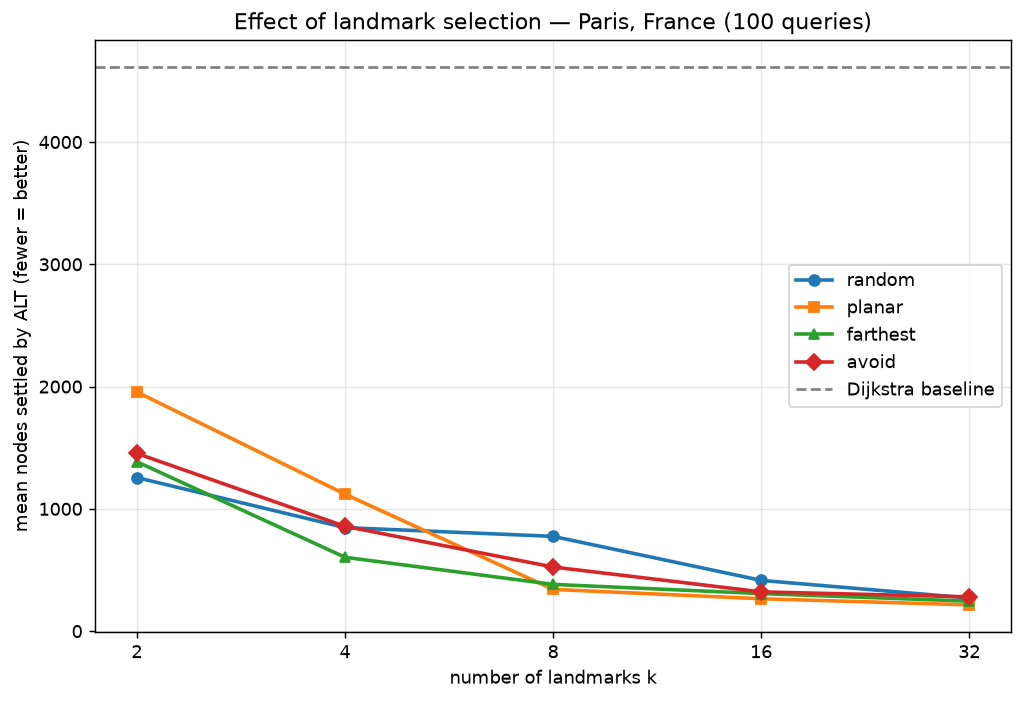
\includegraphics[width=0.85\textwidth]{figures/landmark_study.png}
  \caption[Effet du nombre et du placement des landmarks]{Nœuds explorés par ALT
  en fonction du nombre de landmarks $k$, pour les quatre stratégies de sélection.}
  \label{fig:landmark-study}
\end{figure}

\begin{table}[H]
  \centering
  \small
  \begin{tabular}{@{}lrrrrr@{}}
    \toprule
    Stratégie & $k=2$ & $k=4$ & $k=8$ & $k=16$ & $k=32$ \\
    \midrule
    \texttt{random}   & 1\,256 & 847    & 775 & 415 & 271 \\
    \texttt{planar}   & 1\,956 & 1\,121 & 342 & 265 & 215 \\
    \texttt{farthest} & 1\,386 & 604    & 382 & 307 & 245 \\
    \texttt{avoid}    & 1\,453 & 857    & 524 & 321 & 280 \\
    \bottomrule
  \end{tabular}
  \caption{Nœuds explorés par ALT selon la stratégie et le nombre de landmarks
  (référence Dijkstra $\approx$ 4\,614).}
  \label{tab:landmark-study}
\end{table}

Trois conclusions se dégagent :

\begin{enumerate}
  \item \textbf{Avec peu de landmarks, le placement fait tout.} À $k = 4$,
        \texttt{farthest} explore 604 nœuds contre 847 pour \texttt{random} : des
        landmarks périphériques bien choisis donnent des bornes bien plus fortes
        que le hasard. \texttt{random} a besoin d'environ 4 fois plus de landmarks
        pour égaler l'élagage des stratégies informées.
  \item \textbf{Les rendements décroissent et les stratégies convergent} quand
        $k$ croît : dès $k = 32$, les quatre sont à $\sim 25\,\%$ les unes des
        autres. Sur la forme compacte et à peu près circulaire de Paris,
        \texttt{planar} rivalise avec \texttt{farthest} ; toutes deux dominent
        \texttt{random} dans la plage utile $k = 4\ldots16$.
  \item \textbf{\texttt{avoid} (Goldberg--Werneck) est compétitif sans être un
        vainqueur net ici.} Sa sélection adaptative paie sur de grands réseaux
        irréguliers, mais sur cette petite ville compacte les stratégies purement
        géométriques placent déjà les landmarks quasi optimalement sur la
        frontière, et \texttt{avoid} coûte $\sim 3\times$ plus cher en
        pré-calcul. Résultat honnête : la méthode la plus sophistiquée n'est pas
        automatiquement la meilleure sur une instance facile.
\end{enumerate}

Les cartes de placement (figure~\ref{fig:landmark-maps}) confirment le
mécanisme : \texttt{farthest}, \texttt{planar} et \texttt{avoid} poussent les
landmarks vers la frontière de la ville, là où l'inégalité triangulaire orientée
est la plus serrée, tandis que \texttt{random} gaspille des ancres dans le centre
dense.

\begin{figure}[H]
  \centering
  \subfigure[\texttt{random}]{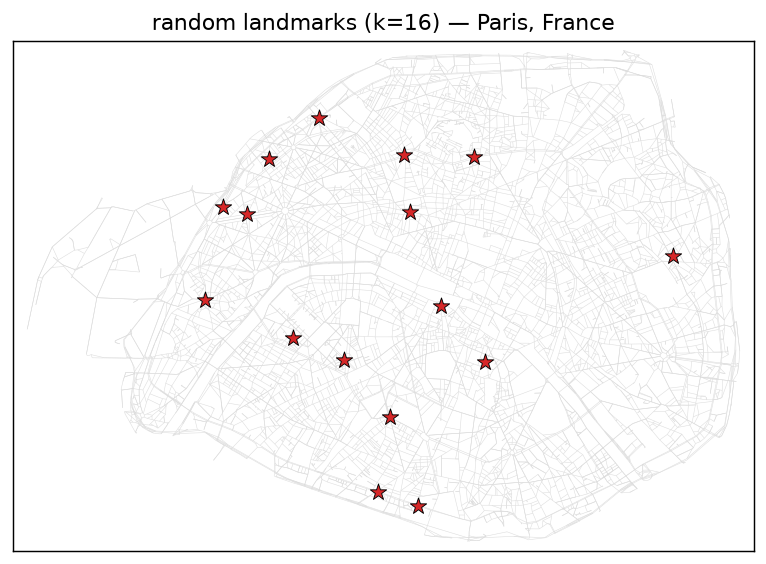
\includegraphics[width=0.46\textwidth]{figures/landmarks_random.png}}\hfill
  \subfigure[\texttt{planar}]{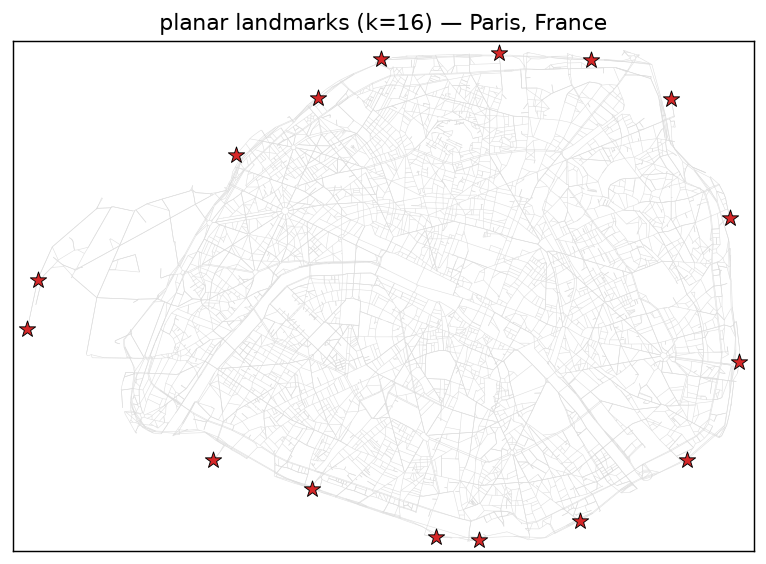
\includegraphics[width=0.46\textwidth]{figures/landmarks_planar.png}}\\[0.3cm]
  \subfigure[\texttt{farthest}]{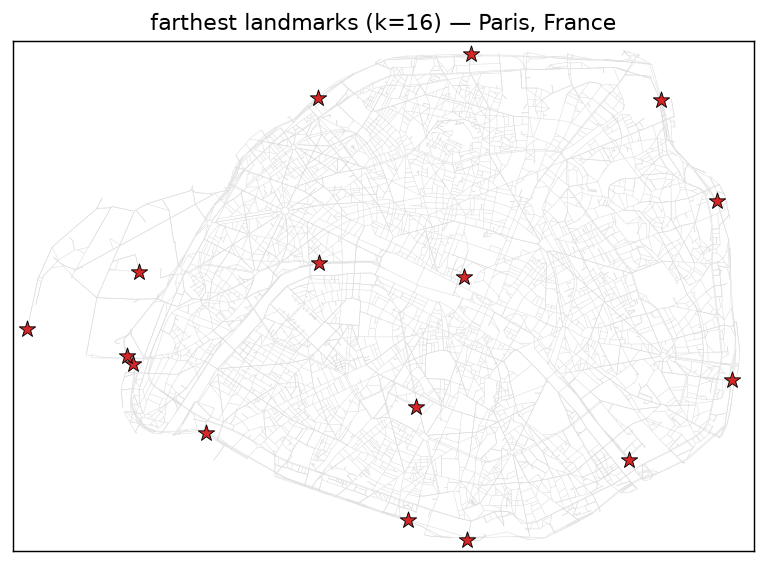
\includegraphics[width=0.46\textwidth]{figures/landmarks_farthest.png}}\hfill
  \subfigure[\texttt{avoid}]{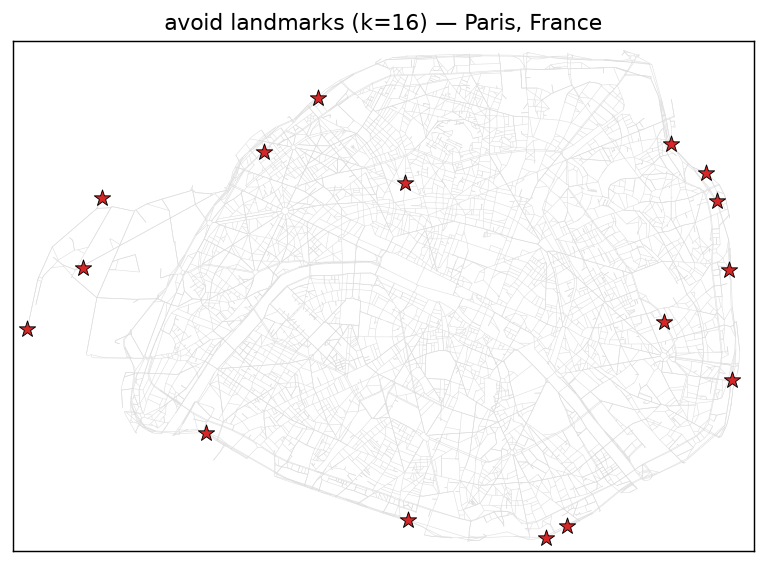
\includegraphics[width=0.46\textwidth]{figures/landmarks_avoid.png}}
  \caption[Placement des landmarks selon la stratégie]{Placement des 16 landmarks
  selon la stratégie. Les stratégies informées (\texttt{planar},
  \texttt{farthest}, \texttt{avoid}) placent les ancres en périphérie ;
  \texttt{random} les disperse, souvent dans le centre dense.}
  \label{fig:landmark-maps}
\end{figure}

\section{Structure de données : file à seaux contre tas binaire}
\label{sec:bucket-result}

Avec la largeur fixée au poids d'arc minimal, la file à seaux de Dial est exacte
(le contrôle d'optimalité passe) et reproduit le tas nœud pour nœud. Dans notre
implémentation Python, elle n'est \emph{pas} plus rapide (8{,}0~ms contre
6{,}5~ms) car le \texttt{heapq} de Python est une extension C tandis que notre
file à seaux est interprétée. C'est cohérent avec les résultats vus en cours, où
les accélérations du tableau de piles sont obtenues avec une implémentation
compilée exploitant la disposition mémoire des seaux : l'\emph{asymptotique}
favorise les seaux, mais les constantes décident en pratique.

\section{Routage multi-étapes et itinéraire lisible}
\label{sec:multistop}

L'exemple fil rouge (\S\ref{sec:filrouge}) est précisément un trajet à étapes :
Dauphine $\to$ PariSanté $\to$ ENS $\to$ PSL. Une route visitant les étapes
\textbf{dans l'ordre donné} se décompose en legs de plus court chemin
indépendants, un par paire consécutive, simplement concaténés. Tout algorithme
ci-dessus s'applique donc inchangé, et ses gains par leg s'additionnent
(table~\ref{tab:multistop}).

\begin{table}[H]
  \centering
  \small
  \begin{tabular}{@{}lrrrrr@{}}
    \toprule
    Algorithme & Dauphine$\to$PS & PS$\to$ENS & ENS$\to$PSL & Total & km \\
    \midrule
    BFS         & 3\,076 & 5\,218 & 878    & 9\,172  & 18{,}61 (non opt.) \\
    DFS         & 513    & 3\,468 & 8\,860 & 12\,841 & \textbf{241{,}55} (non opt.) \\
    Dijkstra    & 3\,674 & 3\,392 & 763    & 7\,829  & 13{,}91 \\
    Greedy      & 69     & 80     & 24     & 173     & 16{,}58 (non opt.) \\
    A*          & 686    & 872    & 157    & 1\,715  & 13{,}91 \\
    ALT         & 414    & 207    & 85     & 706     & 13{,}91 \\
    Bi-Dijkstra & 1\,830 & 2\,607 & 266    & 4\,703  & 13{,}91 \\
    Bi-ALT      & 303    & 150    & 41     & 494     & 13{,}91 \\
    Arc Flags   & 710    & 659    & 479    & 1\,848  & 13{,}91 \\
    \textbf{CH} & 92     & 124    & 79     & \textbf{295} & 13{,}91 \\
    \bottomrule
  \end{tabular}
  \caption{Détail par leg du trajet fil rouge (3 legs, 13{,}91~km au total).
  Nœuds réglés par leg et total.}
  \label{tab:multistop}
\end{table}

Les sept algorithmes optimaux rendent la route identique de 13{,}91~km ; les CH
règlent le moins de nœuds (26{,}5$\times$ moins que Dijkstra). DFS est le
contre-exemple édifiant : sa route combinée fait \textbf{241~km} (18$\times$
l'optimum), traversant la ville en tous sens.

\paragraph{Frontière de modélisation.} Ce découpage tient parce que l'ordre de
visite est \emph{fixé}. Si l'on était libre de choisir l'ordre des étapes, le
problème deviendrait un problème d'ordonnancement de type voyageur de commerce
(NP-difficile) superposé aux calculs de plus courts chemins. Le routage
multi-étapes à ordre fixe reste dans le régime « facile » (polynomial) ; seul
l'ordre le rend difficile.

\paragraph{Itinéraire « tourne à gauche / à droite ».} Les algorithmes rendent le
chemin comme une suite d'intersections, déjà la route exacte (la ligne rouge).
Pour la rendre lisible (une vraie sortie GPS), on conserve le nom de rue OSM de
chaque arc et l'on regroupe les tronçons consécutifs de même rue, en utilisant le
cap géographique entre nœuds pour étiqueter chaque changement de rue en
gauche / droite / tout droit / demi-tour. Pour le premier leg, cela donne par
exemple : \emph{Boulevard Lannes (547~m) $\to$ Rue de Boulainvilliers (671~m)
$\to$ Quai André Citroën (859~m) $\to \dots \to$ Rue d'Oradour-sur-Glane}, soit
5{,}36~km en 23 étapes. Une carte HTML interactive (folium/Leaflet) rend en outre
la route sur un fond de plan réel, une couleur par leg, avec marqueurs de virage
cliquables et panneau récapitulatif : la « vue GPS » du même chemin optimal.

\section{Contraction Hierarchies : le point d'orgue}
\label{sec:ch-result}

Les CH attaquent l'échelle sous un autre angle qu'ALT : au lieu d'une meilleure
heuristique, elles changent le graphe. Sur Paris, le pré-calcul a ajouté
\textbf{31\,328 raccourcis} en $\sim 7$~s, après quoi les requêtes ne règlent que
\textbf{175 nœuds en moyenne, 26{,}9$\times$ moins que Dijkstra, le moins de
tous}. Toutes les distances rendues coïncident exactement avec Dijkstra, et le
vrai chemin est recouvré en dépaquetant récursivement les raccourcis.

En Python pur, le temps réel des CH (0{,}77~ms) est un cheveu supérieur à celui de
Bi-ALT (0{,}56~ms), car chaque pas des CH fait plus de comptabilité qu'une
relaxation simple. C'est un artefact de constante sur petit graphe : l'avantage
des CH croît avec la taille, ce qui explique pourquoi ce sont elles, et non ALT,
qu'utilisent les planificateurs de production (p.\,ex.\ OSRM) sur les réseaux
continentaux. C'est le point d'orgue naturel du thème « échelle » du projet : un
investissement de pré-calcul unique achète la plus petite recherche de toutes.

\section{Étude de passage à l'échelle}
\label{sec:scaling}

Une comparaison sur une seule taille de graphe ne suffit pas : l'énoncé porte sur
\textbf{l'échelle}, donc la vraie question est comment chaque algorithme se
comporte quand le réseau grandit. On exécute les mêmes requêtes sur des extraits
concentriques de Paris, de $\sim 900$ à $\sim 49\,000$ nœuds, et l'on trace les
résultats en fonction de la taille (figure~\ref{fig:scaling}).

\begin{figure}[H]
  \centering
  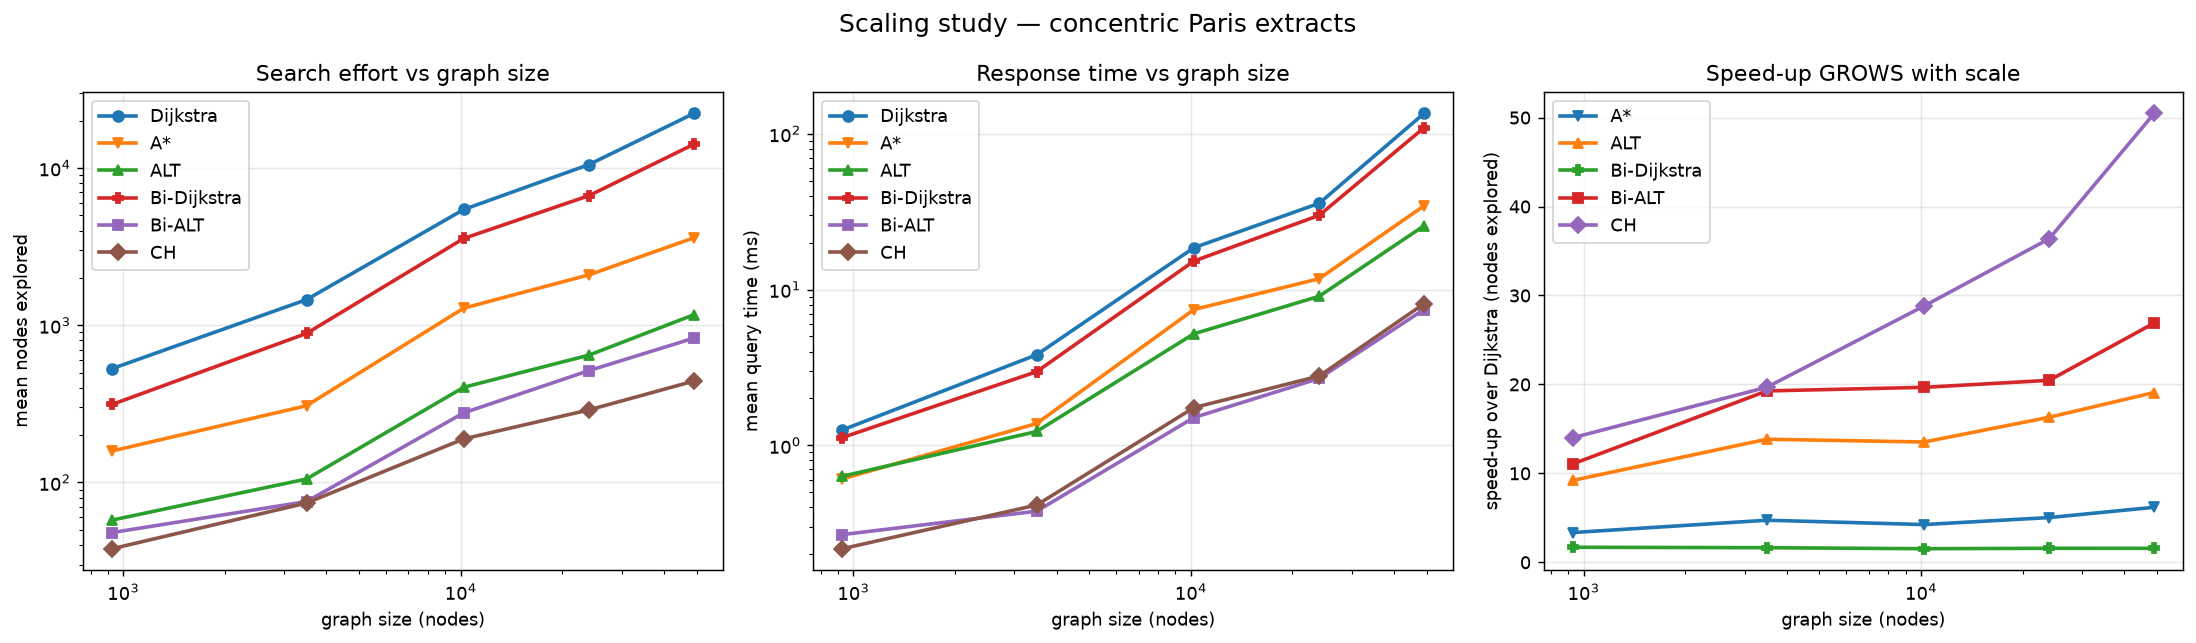
\includegraphics[width=\textwidth]{figures/scaling_study.png}
  \caption[Étude de passage à l'échelle]{Passage à l'échelle sur des extraits
  concentriques de Paris. À gauche : nœuds explorés ; au centre : temps de
  requête ; à droite : accélération sur Dijkstra. L'accélération \emph{croît} avec
  la taille du graphe.}
  \label{fig:scaling}
\end{figure}

\begin{table}[H]
  \centering
  \small
  \begin{tabular}{@{}rrrrr@{}}
    \toprule
    Nœuds & A* & ALT & Bi-ALT & CH \\
    \midrule
    928       & 3{,}3$\times$ & 9{,}1$\times$  & 11{,}0$\times$ & 13{,}9$\times$ \\
    3\,492    & 4{,}7$\times$ & 13{,}9$\times$ & 19{,}1$\times$ & 19{,}7$\times$ \\
    10\,208   & 4{,}2$\times$ & 13{,}5$\times$ & 19{,}7$\times$ & 28{,}8$\times$ \\
    23\,992   & 5{,}0$\times$ & 16{,}3$\times$ & 20{,}5$\times$ & 36{,}4$\times$ \\
    \textbf{49\,045} & 6{,}2$\times$ & 19{,}1$\times$ & 26{,}9$\times$ & \textbf{50{,}5$\times$} \\
    \bottomrule
  \end{tabular}
  \caption{Accélération sur Dijkstra (nœuds explorés) selon la taille du graphe.}
  \label{tab:scaling}
\end{table}

C'est le résultat central du projet. Les algorithmes avancés ne sont pas
« un peu plus rapides » : leur avantage \textbf{se compose avec la taille},
exactement comme le prédit la théorie. Sur le graphe de 49\,000 nœuds, Dijkstra
explore 22\,257 nœuds (135~ms) tandis que les CH en explorent 441 (8~ms).
Fait crucial, à cette échelle le bémol de la « constante Python »
(\S\ref{sec:ch-result}) \textbf{disparaît} : les CH sont $\sim 17\times$ plus
rapides que Dijkstra en temps réel, pas seulement en nombre de nœuds. En
extrapolant la courbe vers les « centaines de milliers de nœuds » de l'énoncé,
l'écart atteint deux ordres de grandeur : d'où le pré-calcul des vrais moteurs.

\section{Analyse statistique de la difficulté des requêtes}
\label{sec:distribution}

Les moyennes masquent la dispersion. On examine donc la \textbf{distribution} de
l'effort sur 300 requêtes et sa dépendance à la longueur du trajet
(figure~\ref{fig:distribution}).

\begin{figure}[H]
  \centering
  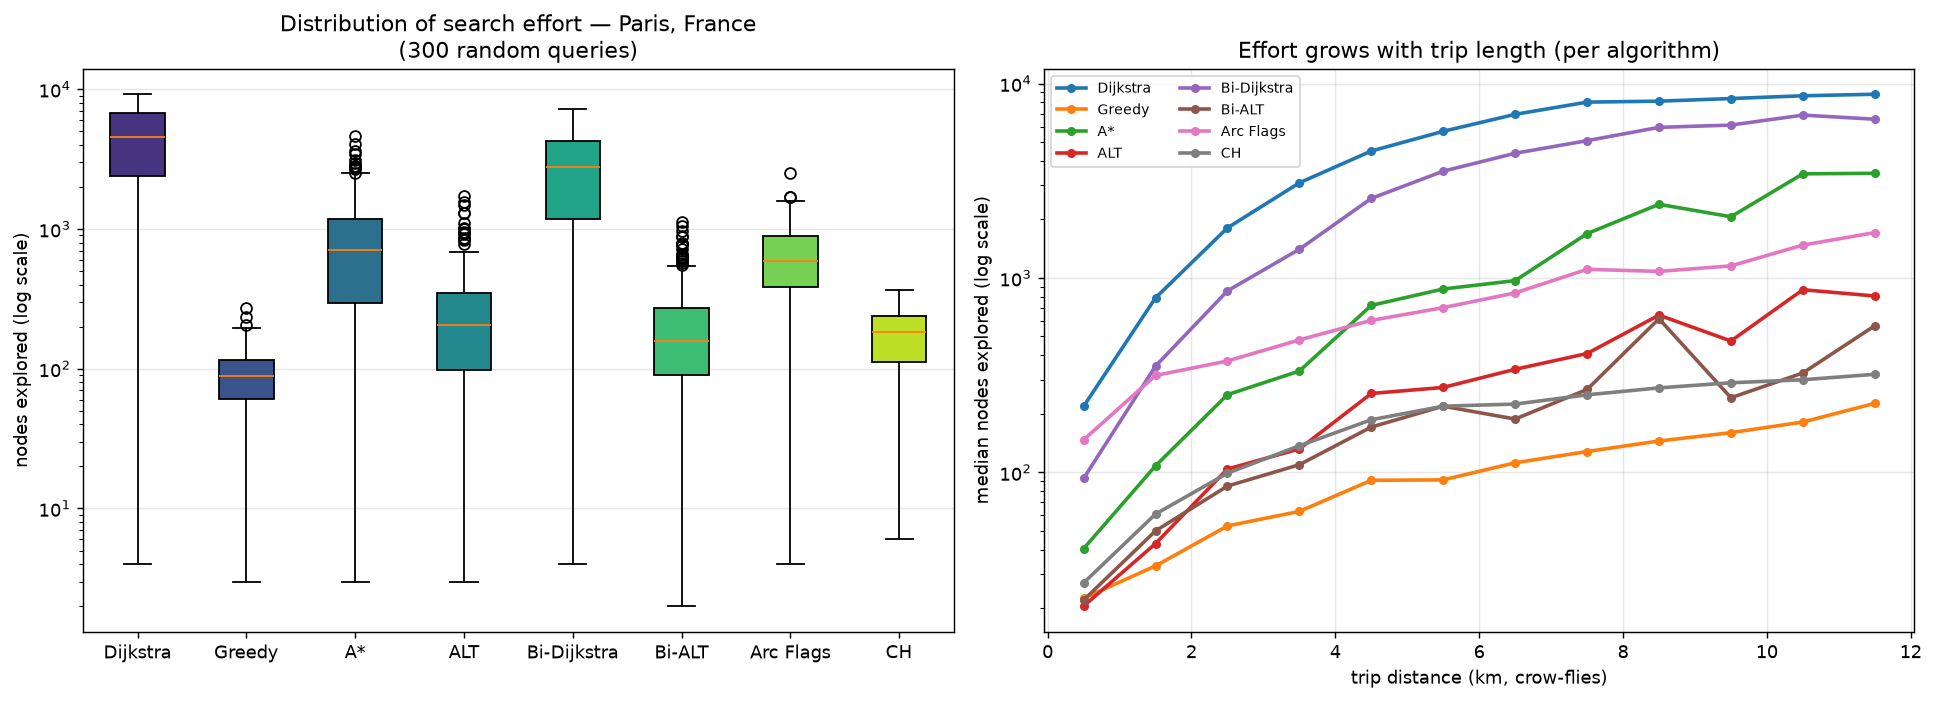
\includegraphics[width=\textwidth]{figures/query_distribution.png}
  \caption[Distribution de l'effort de recherche]{À gauche : boîtes à
  moustaches des nœuds explorés (échelle log) par algorithme : dispersion,
  médiane, valeurs extrêmes. À droite : nœuds explorés médians par bande de
  1~km de distance à vol d'oiseau, une courbe par algorithme.}
  \label{fig:distribution}
\end{figure}

\begin{table}[H]
  \centering
  \small
  \begin{tabular}{@{}lrrrrr@{}}
    \toprule
    Strate & Dijkstra & A* & ALT & Bi-ALT & CH \\
    \midrule
    $< 2$ km   & $\sim$1\,700 & 110    & 70  & 60  & 100 \\
    $2$--$5$ km  & $\sim$3\,900 & 470    & 190 & 150 & 180 \\
    $5$--$10$ km & 6\,968       & 1\,196 & 339 & 250 & 236 \\
    \bottomrule
  \end{tabular}
  \caption{Nœuds explorés médians, stratifiés par distance à vol d'oiseau.}
  \label{tab:distribution}
\end{table}

Deux observations. D'abord, \textbf{l'effort croît avec la longueur du trajet
pour tous les algorithmes, mais à des rythmes très différents} : la recherche de
Dijkstra enfle avec la distance (le panneau de droite le montre saturant près du
graphe entier pour les longs trajets), tandis que les CH restent quasi plates.
Ensuite, \textbf{les CH ne sont pas seulement les plus petites mais les plus
prévisibles} : sur les 300 requêtes, leurs nœuds explorés vont de 6 à 367
(médiane 182), contre 4 à 9\,206 pour Dijkstra. Cette distribution serrée et
insensible à la distance, pas seulement une bonne moyenne, est ce qui rend
le routage hiérarchique fiable en pratique.
